\documentclass[conference,10pt]{IEEEtran}

\usepackage[ansinew]{inputenc}
\usepackage[T1]{fontenc}
\usepackage{amsmath}
\usepackage{amssymb}
%\usepackage{graphicx}
\usepackage{float}
\usepackage{cite}
%\usepackage{epsfig,psfrag}
\usepackage{subfigure}
\usepackage{yfonts}


\newtheorem{theorem}{Theorem}
\newtheorem{corollary}{Corollary}

\newcommand{\eref}[1]{(\ref{#1})}
\newcommand{\fref}[1]{Fig.~\ref{#1}}



\def\rec{\rm rec}
\def\inv{\rm inv}
\def\iDC{$i_{\rm DC}$}
\def\rot{A}

\def\rmL{\ell}
\def\rmC{{\rm c} }
\def\rmd{\rm d}
\def\rmo{\rm o}
\def\rmp{\rm p}
\def\rms{\rm s}
\def\Ts{ T_{\rm s}}
\def\Np{ N_{\rm p}}
\def\rmDC{ {\rm dc}}

\def\mA{\mathcal{A}}
\def\mB{\mathcal{B}}
\def\mC{\mathcal{C}}
\def\mD{\mathcal{D}}
\def\mF{\mathcal{F}}
\def\mI{\mathcal{I}}
\def\mL{\mathcal{L}}
\def\mM{\mathcal{M}}
\def\mQ{\mathcal{Q}}
\def\mR{\mathcal{R}}
\def\mU{\mathcal{U}}
\def\mV{\mathcal{V}}
\def\mW{\mathcal{W}}
\def\mX{\mathcal{X}}

\newlength{\mybox}
\setlength{\mybox}{3.8cm}
\newcommand{\vect}[1]{\boldsymbol{#1}}
\newcommand{\mat}[1]{\boldsymbol{#1}}
\newcommand{\legendevert}[1]{\rotatebox{90}{\fbox{\parbox{\mybox}{\centering #1}}}}
\renewcommand{\legendevert}[1]{\rotatebox{90}{{\parbox{\mybox}{\centering #1}}}}
\newlength{\myraiseh}
\newcommand{\unitvert}[1]{\raisebox{\myraiseh}{\legendevert{\footnotesize{#1}}}}
\def\refframe{{f}}
\def\rotorrefframe{{r}}
\def\statorrefframe{{s}}
\newcommand{\rotor}{^{r}}
\newcommand{\stator}{^{s}}



\bibliographystyle{unsrt}



%
\ifCLASSINFOpdf
  
v\else
  
\fi
% epslatex.pdf at: http://www.ctan.org/tex-archive/info/



% correct bad hyphenation here
\hyphenation{op-tical net-works semi-conduc-tor}


\usepackage{color}	% required for `\textcolor' (yatex added)
\usepackage[dvipdfmx]{graphicx}
\begin{document}
%
% paper title
% can use linebreaks \\ within to get better formatting as desired


\title{Model Based Optimal Tuning of Proportional Resonant Controllers}


% author names and affiliations
% use a multiple column layout for up to three different
% affiliations

\author{\IEEEauthorblockN{Topic number: 5}
\IEEEauthorblockA{  } 
\IEEEauthorblockE{}}
% author names go here

% conference papers do not typically use \thanks and this command
% is locked out in conference mode. If really needed, such as for
% the acknowledgment of grants, issue a \IEEEoverridecommandlockouts
% after \documentclass

% for over three affiliations, or if they all won't fit within the width
% of the page, use this alternative format:
% 
%\author{\IEEEauthorblockN{Michael Shell\IEEEauthorrefmark{1},
%Homer Simpson\IEEEauthorrefmark{2},
%James Kirk\IEEEauthorrefmark{3}, 
%Montgomery Scott\IEEEauthorrefmark{3} and
%Eldon Tyrell\IEEEauthorrefmark{4}}
%\IEEEauthorblockA{\IEEEauthorrefmark{1}School of Electrical and Computer Engineering\\
%Georgia Institute of Technology,
%Atlanta, Georgia 30332--0250\\ Email: see http://www.michaelshell.org/contact.html}
%\IEEEauthorblockA{\IEEEauthorrefmark{2}Twentieth Century Fox, Springfield, USA\\
%Email: homer@thesimpsons.com}
%\IEEEauthorblockA{\IEEEauthorrefmark{3}Starfleet Academy, San Francisco, California 96678-2391\\
%Telephone: (800) 555--1212, Fax: (888) 555--1212}
%\IEEEauthorblockA{\IEEEauthorrefmark{4}Tyrell Inc., 123 Replicant Street, Los Angeles, California 90210--4321}}



\maketitle


\begin{abstract}
The paper considers the optimal choice of gains of proportional-resonant controllers. A converter, controlled in closed loop, but with out proportional resonant controllers, is modeled as a second order transfer function from reference to output. The error between reference and output is fed back through a set of N proportional resonant controller and is added to the reference. The root locus of the closed loop system is considered as a function of the proportional-resonant gains. To find the optimal choice of gains, we consider maximizing the damping of the mode with smallest damping. This corresponds to solving a nonlinear min-max problem. After linearization and reformulation, the problem is stated as a linear program.



\end{abstract}





\IEEEpeerreviewmaketitle


\section{Introduction}

 Proportional resonant tuning methods \cite{568021,6184594,6153368,5338054,6870109,993175,5398914 }




\section{Converter Model}


We consider a voltage source inverter which is assumed to operate in closed loop, but without PR controllers of integrators.  The voltage source inverter is modeled by a second order transfer function which maps the (sinusoidal) reference to the output.;
\begin{align}
\label{eq:InvMdl}
y = G(s)y_{\rm ref},\quad G(s) = \frac{\omega^2}{s^2+\xi\omega s + \omega^2}
\end{align}
where $\omega$ is the natural frequency and $\xi$ is the damping of the (closed loop) inverter.

We note that, with properly designed control, most inverter with resonant filters are expected to behave as second order systems in closed loop. Assuming a system model on the form~(\ref{eq:InvMdl}) is thus not restrictive.



\subsection{Proportional-resonant controllers}

To achieve offset free tracking of the sinusoidal reference $y_{\rm ref}$ and to reduce harmonics in the output, we consider adding proportional-resonant (PR) controllers~\cite{fukuda2001novel} to the system~(\ref{eq:InvMdl}).
The PR controllers are added in a slower outer loop (see Fig.~\ref{fig:}) and adjust the reference according to
\begin{align*}
\tilde{y}_{\rm ref} = y_{\rm ref} + \sum_{n\in\{1,3,5,\dots\}}H_n(s)(y-y_{\rm ref})
\end{align*}
where 
\begin{align*}
H_n(s) = \frac{\lambda_ns}{s^2 - n\omega^2_0}
\end{align*}
where the fundamental frequency $\omega_0$ is the frequency of the reference (typically corresponding to 50 or 60 Hz), and where $\lambda_n$ are the feedback gains of the PR controllers. These gains are tuning parameters who's value affect the transient response of the closed loop system.




\subsection{Closed loop system}

The order of the closed loop system dynamics is $2+2N$ where $N$ is the number of PR controllers added in the outer loop. 




\section{Controller Gain Optimization}

The PR gains $\lambda_n$ affect both the poles and zeros of the closed loop system. In the approach presented below, we focus on the poles and seek to maximize the damping of the (complex) pole pair which has the lowest damping.

To clarify the approach we  consider an example: Consider the case where two PR controllers (with harmonics number $1$ and $3$) are included in the control loop. For this case the system has $6$ poles, and their position in the complex plane is determined by  two gains $\lambda_1$, $\lambda_3$. 

We enumerate combinations of gains $\lambda_1$, $\lambda_3$ and plot the resulting poles, the results is shown by the green dots in Fig.~\ref{fig:PoleExample}. In this figure we also plot the poles obtained when both gains are small (close to zero), and the poles obtained with one particular choice of high gains. The poles obtained with low and high gains are shown by blue and red circles´, respectively.

From Fig.~\ref{fig:PoleExample} it can be seen that one pole pairs moves to the right, closer to the imaginary line (and unstable domain), while the other two pole pairs move left. For sufficiently high gains, one pole pair become two purely real poles, one of which move left and the other move right, into the unstable domain. 
%-----------------------------------------
\begin{figure}[!h]
\centering
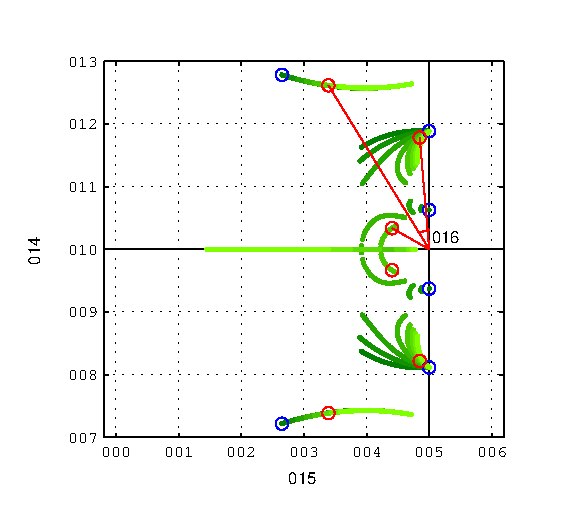
\includegraphics{fig/root_locus_2D}
\caption{Poles of the closed loop system with $N=2$ PR controllers: The green points show poles for various combinations of gains $\lambda_1$, 
$\lambda_3$. Blue circles chow the poles for low gains. Red circle show poles for high gains. }
\label{fig:PoleExample}
\end{figure}
%-----------------------------------------



Since changes in one gain affects all poles, it is not obvious how to choose the gains optimally. Increase in one gain may make one pole pair ``more stable'', but may have negative effects one another pole pair.

To address the problem of how to chose the PR gains, we propose to formulate a max-min optimization problem where we maximize the damping of the least damped pole. More precisely, we consider the angle between of the pole and the imaginary axis (assuming the pole is in the  open left hand plane);
\begin{align*}
\alpha_i = \tan^{-1}(-{\rm real}(p_i) / {\rm imag}(p_i))
\end{align*}
where $p_i$ is a pole in the fourth quadrant. The problem we ideally ant to solve is
\begin{align}
\label{eq:MaxMinProb}
\max_{\lambda_1,\lambda_3,\dots\lambda_N}\min_{i\in \{1,3,\dots,N\}} \alpha_i(\lambda_1,\lambda_3,\dots\lambda_N).
\end{align}
We note that the angles $\alpha_i$ are dependent on the PR gains $\lambda_i$, and that as hte gains vary, different angles take on the role of being ``the smallest''. 



\subsection{Problem approximation}

To obtain a tractable solution, we proceed to approximate $\alpha_i(\lambda_1,\lambda_3,\dots\lambda_N)$ with affine functions of the gains $\lambda_i$: That is, the angles are approximated by
\begin{align}
\label{eq:AngleApprox}
\tilde{\alpha}_i(\lambda_1,\lambda_3,\dots\lambda_N)
= a_i^T\lambda + b_i
\end{align}
where 
\begin{align*}
\lambda = 
\begin{bmatrix}
\lambda_1 & \lambda_3 & \dots & \lambda_N 
\end{bmatrix}^T 
\end{align*}
is a vector containing the gains and where $a_i\in\mathbb{R}^N$, $b_i\in\mathbb{R}$ are constant vectors obtained by sampling the value of the angles
$\alpha_i$ for a number of gain combinations, and performing a least squares fit.



By describing the angles in~(\ref{eq:MaxMinProb}) 
with the approximation~(\ref{eq:AngleApprox}), we obtain a max-min problem with affine cost function. This problem can be equivalently formulated a linear program (LP) according to
\begin{align}
\label{eq:MaxMinProbApprox}
\min c^Tx,\quad {\rm s.t.} Ax\le B
\end{align}
with matrices
\begin{align*}
A = 
\begin{bmatrix}
1 & -c^T_1\\
1 & -c^T_2\\
 & \vdots \\
1 & -c^T_N
\end{bmatrix},\quad 
B =
\begin{bmatrix}
b_1\\
b_2\\
\vdots \\
b_N
\end{bmatrix},\quad 
C =
\begin{bmatrix}
-1\\
0\\
\vdots \\
0
\end{bmatrix}.
\end{align*}
{\bf Put derivation in appendix}




\section{Numerical Example}




\bibliography{IPECrefs}

% that's all folks
\end{document}


